% Created by tikzDevice version 0.10.1 on 2016-09-01 15:51:41
% !TEX encoding = UTF-8 Unicode
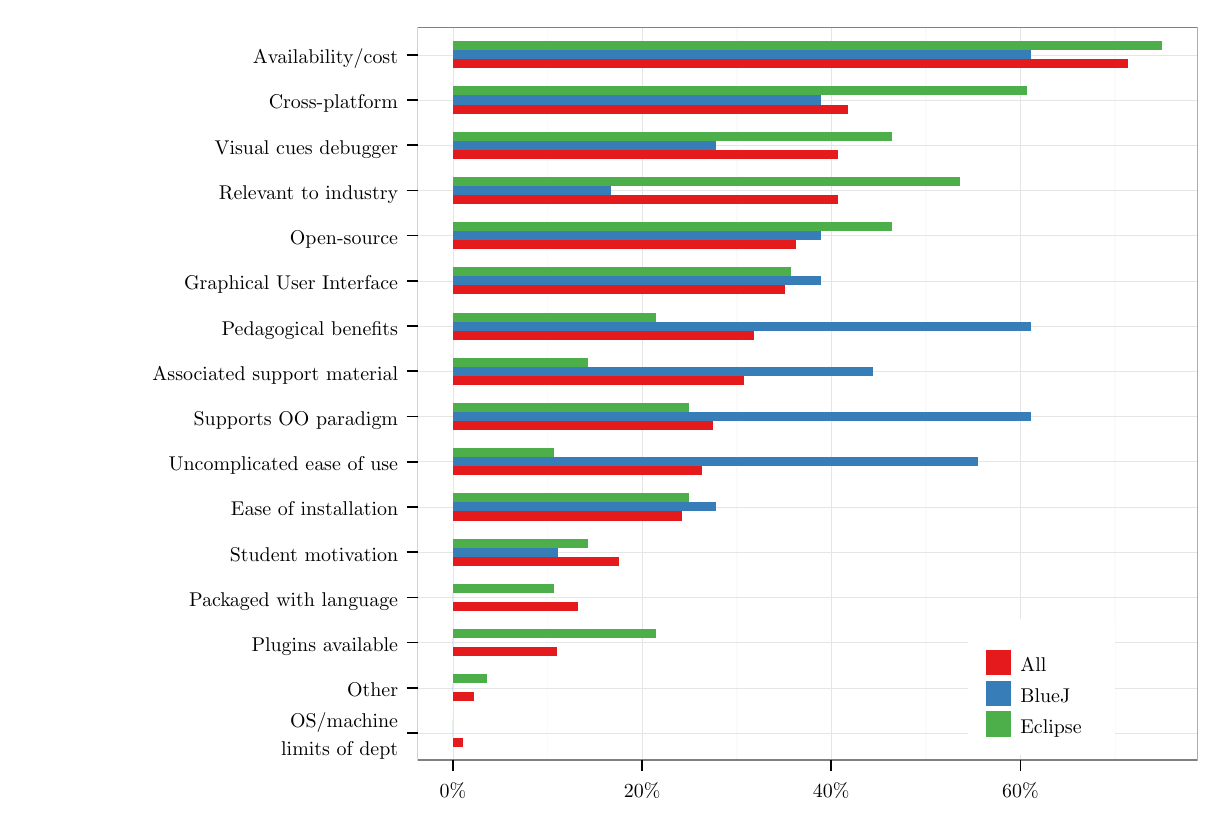
\begin{tikzpicture}[x=1.3pt,y=1.3pt]
\definecolor{fillColor}{RGB}{255,255,255}
\path[use as bounding box,fill=fillColor,fill opacity=0.00] (0,0) rectangle (325.21,216.81);
\begin{scope}
\path[clip] (  0.00,  0.00) rectangle (325.21,216.81);
\definecolor{drawColor}{RGB}{255,255,255}
\definecolor{fillColor}{RGB}{255,255,255}

\path[draw=drawColor,line width= 0.6pt,line join=round,line cap=round,fill=fillColor] (  0.00,  0.00) rectangle (325.21,216.81);
\end{scope}
\begin{scope}
\path[clip] (108.36, 13.20) rectangle (325.21,216.81);
\definecolor{fillColor}{RGB}{255,255,255}

\path[fill=fillColor] (108.36, 13.20) rectangle (325.21,216.81);
\definecolor{drawColor}{gray}{0.98}

\path[draw=drawColor,line width= 0.6pt,line join=round] (144.51, 13.20) --
	(144.51,216.81);

\path[draw=drawColor,line width= 0.6pt,line join=round] (197.08, 13.20) --
	(197.08,216.81);

\path[draw=drawColor,line width= 0.6pt,line join=round] (249.65, 13.20) --
	(249.65,216.81);

\path[draw=drawColor,line width= 0.6pt,line join=round] (302.22, 13.20) --
	(302.22,216.81);
\definecolor{drawColor}{gray}{0.90}

\path[draw=drawColor,line width= 0.2pt,line join=round] (108.36, 20.75) --
	(325.21, 20.75);

\path[draw=drawColor,line width= 0.2pt,line join=round] (108.36, 33.31) --
	(325.21, 33.31);

\path[draw=drawColor,line width= 0.2pt,line join=round] (108.36, 45.88) --
	(325.21, 45.88);

\path[draw=drawColor,line width= 0.2pt,line join=round] (108.36, 58.45) --
	(325.21, 58.45);

\path[draw=drawColor,line width= 0.2pt,line join=round] (108.36, 71.02) --
	(325.21, 71.02);

\path[draw=drawColor,line width= 0.2pt,line join=round] (108.36, 83.59) --
	(325.21, 83.59);

\path[draw=drawColor,line width= 0.2pt,line join=round] (108.36, 96.15) --
	(325.21, 96.15);

\path[draw=drawColor,line width= 0.2pt,line join=round] (108.36,108.72) --
	(325.21,108.72);

\path[draw=drawColor,line width= 0.2pt,line join=round] (108.36,121.29) --
	(325.21,121.29);

\path[draw=drawColor,line width= 0.2pt,line join=round] (108.36,133.86) --
	(325.21,133.86);

\path[draw=drawColor,line width= 0.2pt,line join=round] (108.36,146.43) --
	(325.21,146.43);

\path[draw=drawColor,line width= 0.2pt,line join=round] (108.36,159.00) --
	(325.21,159.00);

\path[draw=drawColor,line width= 0.2pt,line join=round] (108.36,171.56) --
	(325.21,171.56);

\path[draw=drawColor,line width= 0.2pt,line join=round] (108.36,184.13) --
	(325.21,184.13);

\path[draw=drawColor,line width= 0.2pt,line join=round] (108.36,196.70) --
	(325.21,196.70);

\path[draw=drawColor,line width= 0.2pt,line join=round] (108.36,209.27) --
	(325.21,209.27);

\path[draw=drawColor,line width= 0.2pt,line join=round] (118.22, 13.20) --
	(118.22,216.81);

\path[draw=drawColor,line width= 0.2pt,line join=round] (170.79, 13.20) --
	(170.79,216.81);

\path[draw=drawColor,line width= 0.2pt,line join=round] (223.36, 13.20) --
	(223.36,216.81);

\path[draw=drawColor,line width= 0.2pt,line join=round] (275.93, 13.20) --
	(275.93,216.81);
\definecolor{fillColor}{RGB}{228,26,28}

\path[fill=fillColor] (118.22, 16.97) rectangle (121.11, 19.49);
\definecolor{fillColor}{RGB}{77,175,74}

\path[fill=fillColor] (118.22, 22.00) rectangle (118.22, 24.52);
\definecolor{fillColor}{RGB}{55,126,184}

\path[fill=fillColor] (118.22, 19.49) rectangle (118.22, 22.00);
\definecolor{fillColor}{RGB}{228,26,28}

\path[fill=fillColor] (118.22, 29.54) rectangle (124.00, 32.06);
\definecolor{fillColor}{RGB}{77,175,74}

\path[fill=fillColor] (118.22, 34.57) rectangle (127.61, 37.08);
\definecolor{fillColor}{RGB}{55,126,184}

\path[fill=fillColor] (118.22, 32.06) rectangle (118.22, 34.57);
\definecolor{fillColor}{RGB}{228,26,28}

\path[fill=fillColor] (118.22, 42.11) rectangle (147.11, 44.62);
\definecolor{fillColor}{RGB}{77,175,74}

\path[fill=fillColor] (118.22, 47.14) rectangle (174.55, 49.65);
\definecolor{fillColor}{RGB}{55,126,184}

\path[fill=fillColor] (118.22, 44.62) rectangle (118.22, 47.14);
\definecolor{fillColor}{RGB}{228,26,28}

\path[fill=fillColor] (118.22, 54.68) rectangle (152.89, 57.19);
\definecolor{fillColor}{RGB}{77,175,74}

\path[fill=fillColor] (118.22, 59.71) rectangle (146.37, 62.22);
\definecolor{fillColor}{RGB}{55,126,184}

\path[fill=fillColor] (118.22, 57.19) rectangle (118.22, 59.71);
\definecolor{fillColor}{RGB}{228,26,28}

\path[fill=fillColor] (118.22, 67.25) rectangle (164.43, 69.76);
\definecolor{fillColor}{RGB}{77,175,74}

\path[fill=fillColor] (118.22, 72.27) rectangle (155.78, 74.79);
\definecolor{fillColor}{RGB}{55,126,184}

\path[fill=fillColor] (118.22, 69.76) rectangle (147.42, 72.27);
\definecolor{fillColor}{RGB}{228,26,28}

\path[fill=fillColor] (118.22, 79.82) rectangle (181.78, 82.33);
\definecolor{fillColor}{RGB}{77,175,74}

\path[fill=fillColor] (118.22, 84.84) rectangle (183.93, 87.36);
\definecolor{fillColor}{RGB}{55,126,184}

\path[fill=fillColor] (118.22, 82.33) rectangle (191.24, 84.84);
\definecolor{fillColor}{RGB}{228,26,28}

\path[fill=fillColor] (118.22, 92.38) rectangle (187.53, 94.90);
\definecolor{fillColor}{RGB}{77,175,74}

\path[fill=fillColor] (118.22, 97.41) rectangle (146.37, 99.93);
\definecolor{fillColor}{RGB}{55,126,184}

\path[fill=fillColor] (118.22, 94.90) rectangle (264.26, 97.41);
\definecolor{fillColor}{RGB}{228,26,28}

\path[fill=fillColor] (118.22,104.95) rectangle (190.43,107.47);
\definecolor{fillColor}{RGB}{77,175,74}

\path[fill=fillColor] (118.22,109.98) rectangle (183.93,112.49);
\definecolor{fillColor}{RGB}{55,126,184}

\path[fill=fillColor] (118.22,107.47) rectangle (278.85,109.98);
\definecolor{fillColor}{RGB}{228,26,28}

\path[fill=fillColor] (118.22,117.52) rectangle (199.10,120.03);
\definecolor{fillColor}{RGB}{77,175,74}

\path[fill=fillColor] (118.22,122.55) rectangle (155.78,125.06);
\definecolor{fillColor}{RGB}{55,126,184}

\path[fill=fillColor] (118.22,120.03) rectangle (235.03,122.55);
\definecolor{fillColor}{RGB}{228,26,28}

\path[fill=fillColor] (118.22,130.09) rectangle (201.99,132.60);
\definecolor{fillColor}{RGB}{77,175,74}

\path[fill=fillColor] (118.22,135.12) rectangle (174.55,137.63);
\definecolor{fillColor}{RGB}{55,126,184}

\path[fill=fillColor] (118.22,132.60) rectangle (278.85,135.12);
\definecolor{fillColor}{RGB}{228,26,28}

\path[fill=fillColor] (118.22,142.66) rectangle (210.64,145.17);
\definecolor{fillColor}{RGB}{77,175,74}

\path[fill=fillColor] (118.22,147.68) rectangle (212.08,150.20);
\definecolor{fillColor}{RGB}{55,126,184}

\path[fill=fillColor] (118.22,145.17) rectangle (220.44,147.68);
\definecolor{fillColor}{RGB}{228,26,28}

\path[fill=fillColor] (118.22,155.23) rectangle (213.53,157.74);
\definecolor{fillColor}{RGB}{77,175,74}

\path[fill=fillColor] (118.22,160.25) rectangle (240.26,162.77);
\definecolor{fillColor}{RGB}{55,126,184}

\path[fill=fillColor] (118.22,157.74) rectangle (220.44,160.25);
\definecolor{fillColor}{RGB}{228,26,28}

\path[fill=fillColor] (118.22,167.79) rectangle (225.10,170.31);
\definecolor{fillColor}{RGB}{77,175,74}

\path[fill=fillColor] (118.22,172.82) rectangle (259.03,175.33);
\definecolor{fillColor}{RGB}{55,126,184}

\path[fill=fillColor] (118.22,170.31) rectangle (162.04,172.82);
\definecolor{fillColor}{RGB}{228,26,28}

\path[fill=fillColor] (118.22,180.36) rectangle (225.10,182.88);
\definecolor{fillColor}{RGB}{77,175,74}

\path[fill=fillColor] (118.22,185.39) rectangle (240.26,187.90);
\definecolor{fillColor}{RGB}{55,126,184}

\path[fill=fillColor] (118.22,182.88) rectangle (191.24,185.39);
\definecolor{fillColor}{RGB}{228,26,28}

\path[fill=fillColor] (118.22,192.93) rectangle (227.99,195.44);
\definecolor{fillColor}{RGB}{77,175,74}

\path[fill=fillColor] (118.22,197.96) rectangle (277.80,200.47);
\definecolor{fillColor}{RGB}{55,126,184}

\path[fill=fillColor] (118.22,195.44) rectangle (220.44,197.96);
\definecolor{fillColor}{RGB}{228,26,28}

\path[fill=fillColor] (118.22,205.50) rectangle (305.97,208.01);
\definecolor{fillColor}{RGB}{77,175,74}

\path[fill=fillColor] (118.22,210.53) rectangle (315.36,213.04);
\definecolor{fillColor}{RGB}{55,126,184}

\path[fill=fillColor] (118.22,208.01) rectangle (278.85,210.53);
\definecolor{drawColor}{gray}{0.50}

\path[draw=drawColor,line width= 0.6pt,line join=round,line cap=round] (108.36, 13.20) rectangle (325.21,216.81);
\end{scope}
\begin{scope}
\path[clip] (  0.00,  0.00) rectangle (325.21,216.81);
\definecolor{drawColor}{RGB}{0,0,0}

\node[text=drawColor,anchor=base east,inner sep=0pt, outer sep=0pt, scale=  0.72] at (102.96, 22.15) {~OS/machine};

\node[text=drawColor,anchor=base east,inner sep=0pt, outer sep=0pt, scale=  0.72] at (102.96, 14.38) {limits of dept};

\node[text=drawColor,anchor=base east,inner sep=0pt, outer sep=0pt, scale=  0.72] at (102.96, 30.83) {Other};

\node[text=drawColor,anchor=base east,inner sep=0pt, outer sep=0pt, scale=  0.72] at (102.96, 43.40) {Plugins available};

\node[text=drawColor,anchor=base east,inner sep=0pt, outer sep=0pt, scale=  0.72] at (102.96, 55.97) {Packaged with language};

\node[text=drawColor,anchor=base east,inner sep=0pt, outer sep=0pt, scale=  0.72] at (102.96, 68.54) {Student motivation};

\node[text=drawColor,anchor=base east,inner sep=0pt, outer sep=0pt, scale=  0.72] at (102.96, 81.11) {Ease of installation};

\node[text=drawColor,anchor=base east,inner sep=0pt, outer sep=0pt, scale=  0.72] at (102.96, 93.68) {Uncomplicated ease of use};

\node[text=drawColor,anchor=base east,inner sep=0pt, outer sep=0pt, scale=  0.72] at (102.96,106.24) {Supports OO paradigm};

\node[text=drawColor,anchor=base east,inner sep=0pt, outer sep=0pt, scale=  0.72] at (102.96,118.81) {Associated support material};

\node[text=drawColor,anchor=base east,inner sep=0pt, outer sep=0pt, scale=  0.72] at (102.96,131.38) {Pedagogical benefits};

\node[text=drawColor,anchor=base east,inner sep=0pt, outer sep=0pt, scale=  0.72] at (102.96,143.95) {Graphical User Interface};

\node[text=drawColor,anchor=base east,inner sep=0pt, outer sep=0pt, scale=  0.72] at (102.96,156.52) {Open-source};

\node[text=drawColor,anchor=base east,inner sep=0pt, outer sep=0pt, scale=  0.72] at (102.96,169.08) {Relevant to industry};

\node[text=drawColor,anchor=base east,inner sep=0pt, outer sep=0pt, scale=  0.72] at (102.96,181.65) {Visual cues debugger};

\node[text=drawColor,anchor=base east,inner sep=0pt, outer sep=0pt, scale=  0.72] at (102.96,194.22) {Cross-platform};

\node[text=drawColor,anchor=base east,inner sep=0pt, outer sep=0pt, scale=  0.72] at (102.96,206.79) {Availability/cost};
\end{scope}
\begin{scope}
\path[clip] (  0.00,  0.00) rectangle (325.21,216.81);
\definecolor{drawColor}{RGB}{0,0,0}

\path[draw=drawColor,line width= 0.6pt,line join=round] (105.36, 20.75) --
	(108.36, 20.75);

\path[draw=drawColor,line width= 0.6pt,line join=round] (105.36, 33.31) --
	(108.36, 33.31);

\path[draw=drawColor,line width= 0.6pt,line join=round] (105.36, 45.88) --
	(108.36, 45.88);

\path[draw=drawColor,line width= 0.6pt,line join=round] (105.36, 58.45) --
	(108.36, 58.45);

\path[draw=drawColor,line width= 0.6pt,line join=round] (105.36, 71.02) --
	(108.36, 71.02);

\path[draw=drawColor,line width= 0.6pt,line join=round] (105.36, 83.59) --
	(108.36, 83.59);

\path[draw=drawColor,line width= 0.6pt,line join=round] (105.36, 96.15) --
	(108.36, 96.15);

\path[draw=drawColor,line width= 0.6pt,line join=round] (105.36,108.72) --
	(108.36,108.72);

\path[draw=drawColor,line width= 0.6pt,line join=round] (105.36,121.29) --
	(108.36,121.29);

\path[draw=drawColor,line width= 0.6pt,line join=round] (105.36,133.86) --
	(108.36,133.86);

\path[draw=drawColor,line width= 0.6pt,line join=round] (105.36,146.43) --
	(108.36,146.43);

\path[draw=drawColor,line width= 0.6pt,line join=round] (105.36,159.00) --
	(108.36,159.00);

\path[draw=drawColor,line width= 0.6pt,line join=round] (105.36,171.56) --
	(108.36,171.56);

\path[draw=drawColor,line width= 0.6pt,line join=round] (105.36,184.13) --
	(108.36,184.13);

\path[draw=drawColor,line width= 0.6pt,line join=round] (105.36,196.70) --
	(108.36,196.70);

\path[draw=drawColor,line width= 0.6pt,line join=round] (105.36,209.27) --
	(108.36,209.27);
\end{scope}
\begin{scope}
\path[clip] (  0.00,  0.00) rectangle (325.21,216.81);
\definecolor{drawColor}{RGB}{0,0,0}

\path[draw=drawColor,line width= 0.6pt,line join=round] (118.22, 10.20) --
	(118.22, 13.20);

\path[draw=drawColor,line width= 0.6pt,line join=round] (170.79, 10.20) --
	(170.79, 13.20);

\path[draw=drawColor,line width= 0.6pt,line join=round] (223.36, 10.20) --
	(223.36, 13.20);

\path[draw=drawColor,line width= 0.6pt,line join=round] (275.93, 10.20) --
	(275.93, 13.20);
\end{scope}
\begin{scope}
\path[clip] (  0.00,  0.00) rectangle (325.21,216.81);
\definecolor{drawColor}{RGB}{0,0,0}

\node[text=drawColor,anchor=base,inner sep=0pt, outer sep=0pt, scale=  0.72] at (118.22,  2.85) {0\%};

\node[text=drawColor,anchor=base,inner sep=0pt, outer sep=0pt, scale=  0.72] at (170.79,  2.85) {20\%};

\node[text=drawColor,anchor=base,inner sep=0pt, outer sep=0pt, scale=  0.72] at (223.36,  2.85) {40\%};

\node[text=drawColor,anchor=base,inner sep=0pt, outer sep=0pt, scale=  0.72] at (275.93,  2.85) {60\%};
\end{scope}
\begin{scope}
\path[clip] (  0.00,  0.00) rectangle (325.21,216.81);
\definecolor{fillColor}{RGB}{255,255,255}

\path[fill=fillColor] (261.34, 14.69) rectangle (302.35, 52.44);
\end{scope}
\begin{scope}
\path[clip] (  0.00,  0.00) rectangle (325.21,216.81);
\definecolor{fillColor}{RGB}{228,26,28}

\path[fill=fillColor] (266.32, 36.74) rectangle (273.43, 43.85);
\end{scope}
\begin{scope}
\path[clip] (  0.00,  0.00) rectangle (325.21,216.81);
\definecolor{fillColor}{RGB}{55,126,184}

\path[fill=fillColor] (266.32, 28.20) rectangle (273.43, 35.31);
\end{scope}
\begin{scope}
\path[clip] (  0.00,  0.00) rectangle (325.21,216.81);
\definecolor{fillColor}{RGB}{77,175,74}

\path[fill=fillColor] (266.32, 19.67) rectangle (273.43, 26.78);
\end{scope}
\begin{scope}
\path[clip] (  0.00,  0.00) rectangle (325.21,216.81);
\definecolor{drawColor}{RGB}{0,0,0}

\node[text=drawColor,anchor=base west,inner sep=0pt, outer sep=0pt, scale=  0.72] at (275.95, 37.81) {All};
\end{scope}
\begin{scope}
\path[clip] (  0.00,  0.00) rectangle (325.21,216.81);
\definecolor{drawColor}{RGB}{0,0,0}

\node[text=drawColor,anchor=base west,inner sep=0pt, outer sep=0pt, scale=  0.72] at (275.95, 29.28) {BlueJ};
\end{scope}
\begin{scope}
\path[clip] (  0.00,  0.00) rectangle (325.21,216.81);
\definecolor{drawColor}{RGB}{0,0,0}

\node[text=drawColor,anchor=base west,inner sep=0pt, outer sep=0pt, scale=  0.72] at (275.95, 20.74) {Eclipse};
\end{scope}
\end{tikzpicture}
